
\begin{savequote}
There is no truth. There is only perception.
\qauthor{Gustave Flaubert}
\end{savequote}

\chapter[Multiple Culture Annotation]{Multiple Culture Annotation}
\label{ChapterAnnotation}

\thesiscomment{MAIN POINT: Because cultural perception differences are expected to exist, we collect a new cross culture annotation set using crowdsourcing and address the filtering issues to produce three distinct annotation sets that reflect individual annotator's ratings.}

\thesiscomment{WHAT we do}

\thesiscomment{HOW we do it}

\thesiscomment{RESULTS, IMPACT and NOVELTY}

\thesiscomment{Of course, we expect to find cultural differences. Make it clear why this work is necessary despite that.}

%The previous two chapters describe an automatic system that attempts to recognises \ac{NVC} as humans would rate the same signal. 
Humans often disagree as to the meaning that is expressed in a video clip of \ac{NVC}. As discussed in Section \ref{SectionAnalysisOfMeanRatings}, the statistical mean of ratings is used to form a single label for each video clip. If there is significant inter-annotator disagreement in the data, taking the mean is not necessarily valid because the resulting label does not correspond to any specific human or group of human annotators. One of the factors that affects \ac{NVC} signal perception by humans is the cultural background of the observer (see Section \ref{BackgroundWhatFactorsInfluenceNvc}). As the goal of automatic recognition of \ac{NVC} is to produce labels similar to those generated by humans, modelling the specific cultural perception of \ac{NVC} signals will lead to improvement over training a system in one culture and then applying it in a different culture.% that is not reflected in the training data.
%Using multiple groups of annotations, each which produce an independent subjective set of annotations. 

For the purposes of automatic recognition, all previous research has either gathered annotation data from a specific culture or merged annotations from multiple cultures. This is the first study using subjective annotation for machine learning so that cultures were kept as distinct annotation sets. 
%However, this is not the first to use machine learning on subjective data based on distinct annotators; Reidsma and op den Akker \cite{Reidsma2008b} trained annotator specific classifiers based on contextual addressing labels in a meeting social context.

The main contributions of this chapter are:
\begin{itemize}
 \item Annotation data, based on crowdsourcing, that is suitable basis for automatic recognition of human behaviour.
 \item A quantitative analysis of cross cultural annotation data. The data is analysed in terms of quantifying the possible existence and extent of differences between cultural specific perceptions.
\end{itemize}

Research relating to cultural differences and crowdsourcing are discussed in the next section. Section \ref{SectionCrowdSourceDataCollection} describes the Internet based collection of annotation data. This data is filtered to remove uncooperative workers; the filtering method is described in Section \ref{SectionNeedToFilter}. Section \ref{SectionAnalysisOfCultureAnnotation} describes an analysis of the filtered data.

\section{Related Research}
\label{BackgroundCrossCulture}

The field of cross cultural study of emotion was founded by Darwin in 1872 \cite{Darwin2002}, in which he was struck by the remarkable similarity in emotion expression styles across cultures. 
%The books impact was later assessed by Ekman \cite{Ekman2009}, who claimed that Darwin's key contributions were the emphasis of emotions that were discrete entities that were primarily expressed by the face and had limited universality across cultures and species. 
Darwin also pioneered the use of photographs in the study of emotion, and the assessment of emotion by judgement based studies \cite{Ekman2009}. The key role of culture in non-verbal communication was stressed by Hall \cite{Hall1959}, with particular attention to cultural influences of which the expresser is not consciously aware. Ekman modelled the process of differences in emotion expression by proposing culturally specific display rules \cite{Ekman1969}, but claimed that emotion was largely culturally universal, and this universality was particularly evident in a subset of emotions called ``basic emotions'' \cite{Ekman1972}.
% although he also uses the term ``basic emotions'' for his particular discrete emotion/evolutionary view of emotions \cite{Ekman99}. 
There is less evidence for the universality of non-verbal communication but emotion can be a form of communication \cite{Frith2009}, and that component of \ac{NVC} may be partly universal. %Cultural differences exist in both expression and perception of emotion. Experimental work that examines these differences will now be discussed.

% Possibly relevant? definition of basic emotions? \cite{Ortony1988}, 
Cultural differences in expression of emotion and \ac{NVC} have been studied and observed \cite{Matsumoto2006}. Extreme cases of cultural difference in perception include different head motions for agreement and disagreement \cite{Kassabova2008}, and differences in obscene gestures \cite{Knapp2009}. Gaze aversion direction while thinking has cultural differences \cite{McCarthy2006}. Backchannel signals are more frequent in Japanese culture than \acs{US} culture \cite{White1989}. These differences may be significant for an automatic system if it is trained for one culture and deployed in a different culture. Various cross cultural studies have collected observer judgements and each time have found cultural differences. This has included judgements of pictograms \cite{Cho2007} and emotional avatars \cite{Massaro96, Koda2007}. Marsh \etal found that observers could distinguish a person's nationality by their style of emotional expression \cite{Marsh2003}. Japanese observers were found to be more sensitive to context than Westerners in emotion recognition \cite{Masuda2008}. Some universality was found for non-verbal vocalisation of the common Ekman 6 basic emotions but cultural differences were found in non basic emotions \cite{Sauter2009}. Even the process of perception has been seen to have cultural differences: gaze during emotion recognition were found to have different patterns \cite{Jack2009}, which possibly leads to some cultures having difficulty distinguishing certain emotions. All these findings suggest that differences in expression and perception exist but also there is a great deal of commonality between cultures.

%A cross cultural study linked differences in display rule differences to cultural traits \cite{Matsumoto08}

Elfenbein and Ambady \cite{Elfenbein2002b, Elfenbein2002} argued that members of a cultural group are more accurate at recognising emotions in their group, when compared to an out-of-group observer. In response to this paper, Matsumoto argued that for the group hypothesis to be properly tested, the sample sizes needed to be balanced and the stimuli had to be equivalent \cite{Matsumoto2006} and this had not been done. The potential for culturally specific concepts can make \ac{NVC} and emotion words difficult to translate or transfer to new cultures (see Section \ref{SectionTranslationOfInstrument}). If an in-group advantage exists for \ac{NVC}, cultures that differ from the expresser's culture may annotate data differently. This may range from a reduction in inter-annotator agreement to significant misinterpretations of the \ac{NVC} meaning. %While there have been a vast number of cross cultural studies of human behaviour, none have been used as a basis for machine learning of human behaviour recognition.
% This may be that certain concepts are only meaningful within a culture (an ``emic'' account), which contrasts with an observer outside a culture that (an ``etic'' account) \cite{Headland1990}.

Various approaches exist to detect and remove outliers in questionnaire responses \cite{Zijlstra2011}. The method proposed in this chapter differs in that it considers each annotator response set as something to be accepted or rejected as an entirety. This property makes it more suitable to a crowdsourcing application.

%DISCUSS? Inter-annotator disagreements imply bad automatic results? \cite{Reidsma2008Thesis}

\subsection{Crowdsourcing of Annotation Data}

Crowdsourcing refers to the participation of a loosely defined group of people who work towards a common goal, often using the Internet to coordinate the work. Some scientific projects have used crowdsourcing and involving many workers from across the world, including Cooper \etal \cite{Cooper2010}, for ``foldit'' protein folding and Riddick \etal for ``Galaxy Zoo'' \cite{Raddick2010} which generated enough interest to not need payment to incentivise participation. Tarasov \etal \cite{Tarasov2010} proposed using crowdsourcing to gather emotional label annotation data. There are few or no previous works that use crowdsourcing for annotation of \ac{NVC} behaviour, for the purposes of automatic recognition. The next section describes how crowdsourcing was applied to annotation of \ac{NVC} samples.

\section{Data Collection Method}
\label{SectionCrowdSourceDataCollection}

The annotation task involves viewing a series of short views from the corpus (as described in Section \ref{SectionDescriptionOfTwoTalkCorpus}) and providing responses to the questions on \ac{NVC} signals (described in Section \ref{SectionDescribeQuestions}). Computer based annotation is commonly used for annotation because the annotation task can be precisely defined by the experimenter, and because of the convenience of collection and analysis of the results. Computer based annotation may also be conducted remotely, which is cost effective and convenient but provides less control on how the annotators complete the task. Differences in the equipment, the presence or absence of audio and a different physical environment may affect how an annotator perceives an \ac{NVC} signal. These factors could not be controlled using remote computer based annotation and may result in an increase of inter-annotator differences.

%Some tasks are sufficiently interesting as to not require a monetary incentive for annotators to participate. However, given our annotation task is relatively arduous (see Section \ref{BackgroundWhyNvcAnnotationIsBoring}), Internet crowdsourced workers were used and were paid a small fee to complete each annotation task. 
The annotation data was collected from multiple cultures.
Crowdsourced workers may be located anywhere in the world and they use any standards compliant web browser to complete tasks which have been defined by a work supplier. There is usually little screening of workers and no qualification or requirements beyond being able to access the Internet. A typical screen shot of the web page presented to the annotator is shown in Figure \ref{FigureAnnotationSurveyScreenshot}. Although it is quite possible to independently establish a website that enables annotation and payments, there are several web-based services that manage the website infrastructure for a fee. Crowdflower's web service\footnote{\scriptsize{http://crowdflower.com/}} was used to manage the annotation work. This service provides a high level interface to other crowdsourcing services, such as Amazon Mechanical Turk\footnote{\scriptsize{https://www.mturk.com/}} and Samasource\footnote{\scriptsize{http://samasource.org/}}. Each service has an associated worker pool with a distinct worker demographic. However, crowdsourcing has several issues that need consideration if high quality annotation is required.

As previously mentioned, the order of the questions presented to the annotators was randomised to reduce the effect of question order. It was impossible to insert a demographic survey before the users undertook the main task. This was unfortunate, because demographic information may be useful in accounting for inter-annotator differences. However, the IP address of each annotator was available, which was used to assign a rough geographic location of each Internet user. Also, Samasource specialises in refugee populations and an annotators physical location can differ from their cultural background. In particular, a significant response was received from annotators located in Kenya, but these people were likely to be Sudanese refugees. Also, an IP address is not a perfectly reliable method to localise users, given the existence of Internet proxy services. Despite these factors, an IP address based location was considered sufficient for our needs. In the case of refugees, it is not necessary to know the exact culture of origin, as long as the IP address location corresponds to multiple distinct cultural groups. 

Volunteers may be sampled from a sub-group within each culture and this effect is called ``sampling bias''. 
%Computer based tools are used to perform the annotation. 
The availability of skills and equipment varies in each population, therefore if computer use is required, sample bias is likely to occur. The extent of this bias is unknown. It is possible that there is no unified \ac{NVC} perception consensus in a single culture, if any intra-culture factor has a large effect on \ac{NVC} perception. It may therefore be undesirable to sample from an entire country's population, if the annotations within a group are not in agreement. However, using a sub-group of a culture is satisfactory, as long as the sample is not assumed to represent the culture as a whole. If the applications of this technology are to be adopted by a sub-group of a culture, such as those with easy access to computers, this bias may be beneficial in creating a system that operates well with potential users. In conventional surveys, various techniques can be used to improve annotator agreement, such as training, annotators previewing the corpus, panel-based ratings, repeat ratings of a clip by the same annotator. These were not used because of the technical limitations of the present crowd sourcing tools, for which work unit presentation is pseudo-random. Annotator normalisation was not used because the annotation data is sparse and  perception labels of individual annotators is not required for this study, but this technique may be adapted to this situation in future work.

The survey data described in Section \ref{SectionAnalysisOfHumanAnnotation} was collected using unpaid volunteers. This chapter relies on paid workers to provide annotation data. Given that it was possible for an annotator to provide random data in return for a monetary reward, there can be quality control issues which need to be managed. The process for filtering valid work from random annotation is described in Section \ref{SectionNeedToFilter}. The workers that accept to complete the task as instructed are designated as ``trusted'' workers, and annotators that respond with poor data or random data are designated as ``untrusted''. Crowdflower provides its own semi-automatic tool for identifying trusted workers called ``gold'', presumably from the term ``gold standard''. This gold tool was used to reduce expenditure on poor annotation data. However, this tool did not affect the final annotation data and both trusted and untrusted data was retained and filtered using the method described below.

\thesiscomment{Can a simple test question find random responders? Is this better than filtering?}

An alternative approach to identification of trusted workers is to introduce additional validation questions with a known answer. Unfortunately, there are several practical problems with this approach in a crowdsourcing environment. Additional questions increase the amount of work required of the annotators. Due to the current technical limitations of the annotation service, each annotation task or ``work unit'' must have the same number of responses for every question. The basic work unit requires the four \ac{NVC} signal ratings of the questionnaire. To add one more question would increase the workload by 25\%. Also, humans that intend to cheat will be able to identify any validation questions and simply answer them correctly, while randomly answering the \ac{NVC} questions. This possibility of circumventing the validation questions makes their usefulness questionable. The annotation data would still need to be analysed and filtered to provide confidence that the annotation data is valid. The next section discusses the issue of language in the context of \ac{NVC} signal perception ratings.

\subsection{Translation of Cross Cultural Instruments}
\label{SectionTranslationOfInstrument}

The design of the questionnaire was previously discussed in Section \ref{SectionDescribeQuestions} but previously only a single culture and a single language have been considered. 
Different languages are spoken throughout the world with English being the first language for approximately 380 million people \cite{Economist2001}. Second language speakers and learners of English outnumber first language users but the majority of people speak languages other than English. 
The questionnaire was applied to cultures that have significant differences, including language usage. The translation of survey instruments is used in many scientific fields to avoid the instrument being understood differently outside of its original culture. According to Geisinger \cite{Geisinger1994}, an instrument needs to be translated and the fact that the translated instrument measures the same constructs as the original version needs to be verified. A translation may lead to the instrument measuring something other than what was intended \cite{Poyatos1997}, and this makes comparison between cultures problematic. Translation of survey instruments is strongly recommended in medical surveys, using rigorous methods \cite{Gjersing2010, Beaton2000, Morales2001}. Medical surveys contain questions that refer to concepts that are labels for observable phenomena that exist separately from the observer. However, the \ac{NVC} questionnaire is quite different in that the concepts do not exist except as subjective interpretations. The questionnaire asks for an annotator's interpretation of \ac{NVC} signals which depends on their cultural background, etc. The term ``\ac{NVC}'' implies that these communication signals do not directly correspond to word based concepts. De Mendoza \cite{Mendoza2008} argues emotion labels used to express subjective interpretations are not ``defined by necessary and sufficient features'' but rather ``probabilistic concepts with an internal structure with better and worse examples of the category and fuzzy boundaries''. In this view, a particular instance of an emotion might be perceived as mostly agreeing, somewhat blaming, slightly surprised or any other combination of fuzzy overlapping labels. The same can be said of \ac{NVC} signal perception, in that the labels used in the questionnaire are interrelated, fuzzy, partly overlapping and not comprehensive.

% Fernandez-Dols2003 discusses affect to get away from the realism/nominalism problem
% \cite{Davaninezhad2009}
% Translation of survey \cite{Ekman1969} \cite{Haralick1989} \cite{Headland1990} \cite{Marin1991} \cite{Humphrey1993} \cite{Geisinger1994} \cite{Poyatos1997} \cite{Morales2001} \cite{Economist2001} \cite{Fernandez-Dols2003} \cite{Thirumalai2003} \cite{Matsumoto2006} \cite{Cho2007} \cite{Mendoza2008} \cite{Davaninezhad2009} \cite{Gjersing2010} \cite{Noproblem}

Given that an instrument is to be used in multiple cultures, the concepts referred to in the instrument should be consistently understood. There are two approaches that were considered: translating a questionnaire to cultures of interest or to present a single questionnaire in multiple cultures. These approaches will now be discussed in more detail.

If the concepts referred to exist only in the mind of an observer, these concepts might be ``cultural concepts'' that do not necessarily exist in another language or culture. Because no one-to-one mapping exists between different cultural concepts, the translation of instruments and cross culture recognition are problematic \cite{Elfenbein2002}. There are many examples of emotional concepts that do not have direct translations (\textit{verg\"{u}enza} from Spanish to English, \textit{shimcheong} from Korean to English \cite{Mendoza2008}). Applying this to \ac{NVC}, a particular communication action may be perceived in Spain as a particular combination of cultural concepts but in the United Kingdom, a different combination of cultural concepts. With this culturally specific mapping between concept labels and experiences, a perfect one-to-one mapping will be impossible. Therefore, cultural differences could be caused by imperfect translation leading to different cultural concepts used by the annotators or the way emotions are mapped onto the cultural concepts, with no easy way to distinguish these two effects. 

The other approach is to present the same questionnaire in multiple cultures. The words in the questionnaire would be interpreted by the annotators in relation to their own cultural concepts and this can change the basis by which an annotator perceives and evaluates \ac{NVC} signals. %Cultural differences could cause language understanding differences, in turn leading to differences the cultural concepts used by the annotators, or the way emotions are mapped onto the cultural concepts, and as with a translated survey, with no easy way to distinguishing between these two effects.

Given both approaches have problems, the latter option of having a single survey in one language presented to multiple cultures was used. This decision was based on the fact that, given the crowdsourcing tools available at the time, a specific group of annotators could not be targeted by a tailored questionnaire, although this was planned in a future version of the tools. It may be possible to create a questionnaire using word clouds that would lend themselves better to probabilistic translation (e.g. English word cloud to Spanish word cloud). Given all these considerations, the transfer of everyday concepts from one culture to another is complex and a subject worthy of further study. The next section takes the collected annotation data and considers how untrusted annotators can be identified and removed from the data set.

\section{Filtering Untrusted Workers}
\label{SectionNeedToFilter}

\thesisstatement{Internet worker annotation is noisy, but trusted workers can be found by filtering the data}

\begin{figure}
\centering
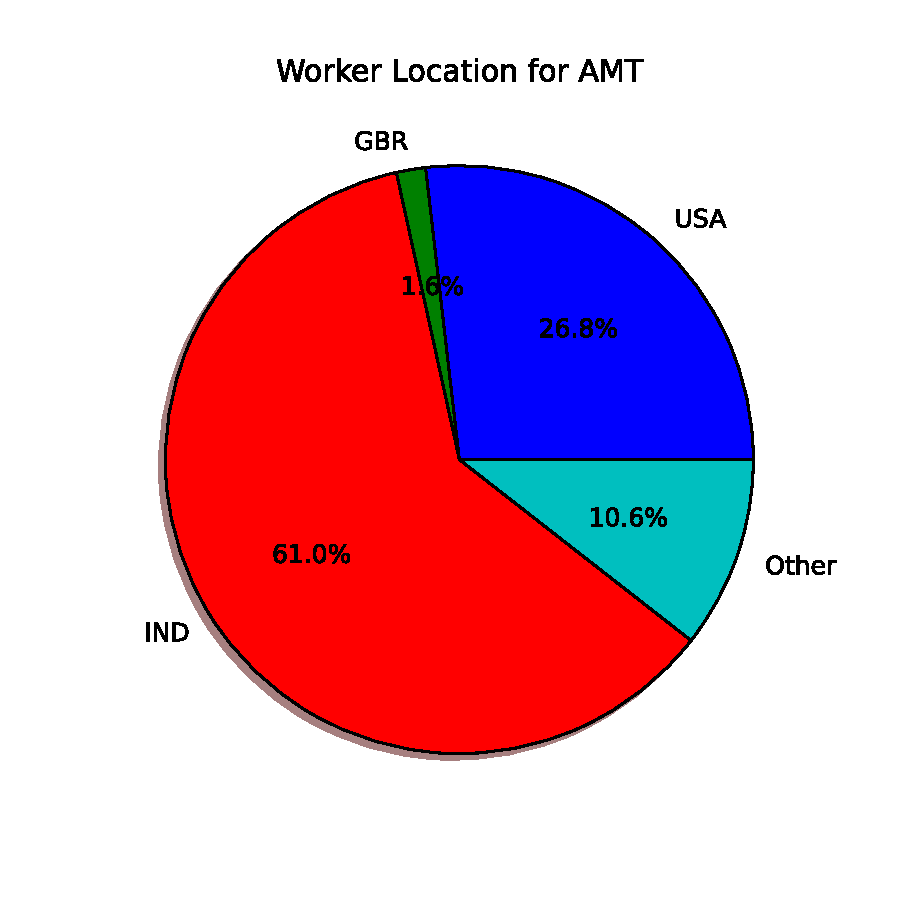
\includegraphics[width = 0.32 \columnwidth]{annotation/demog-amt.pdf}
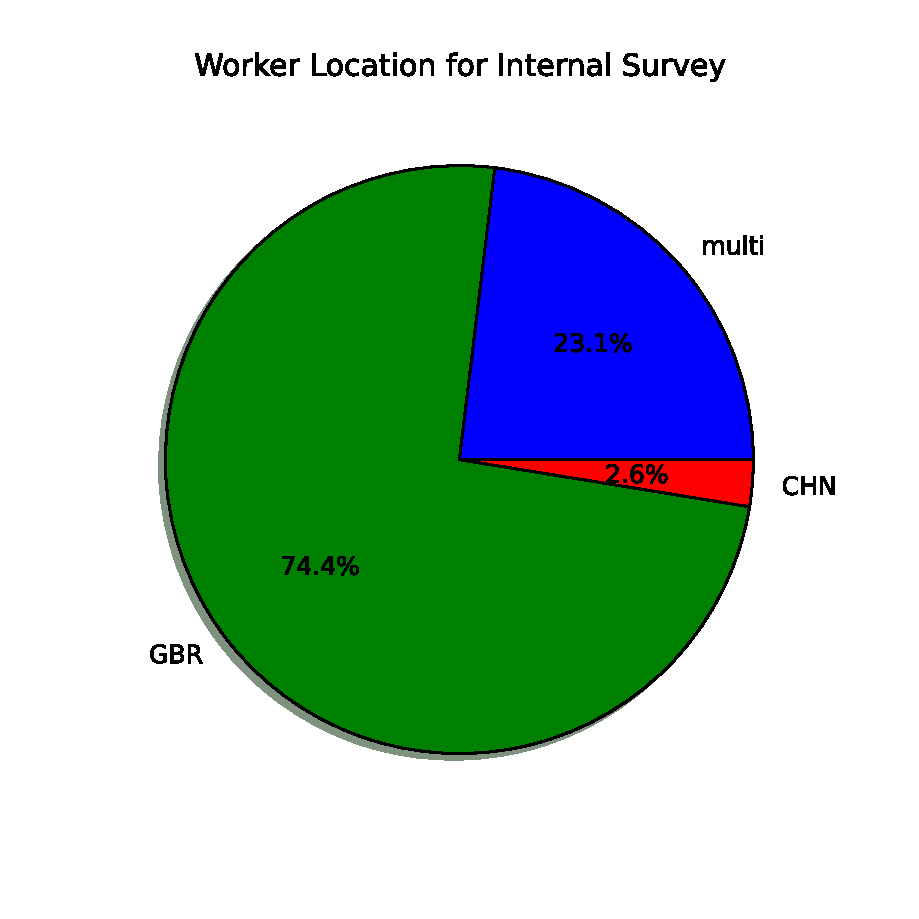
\includegraphics[width = 0.32 \columnwidth]{annotation/demog-internal.pdf}
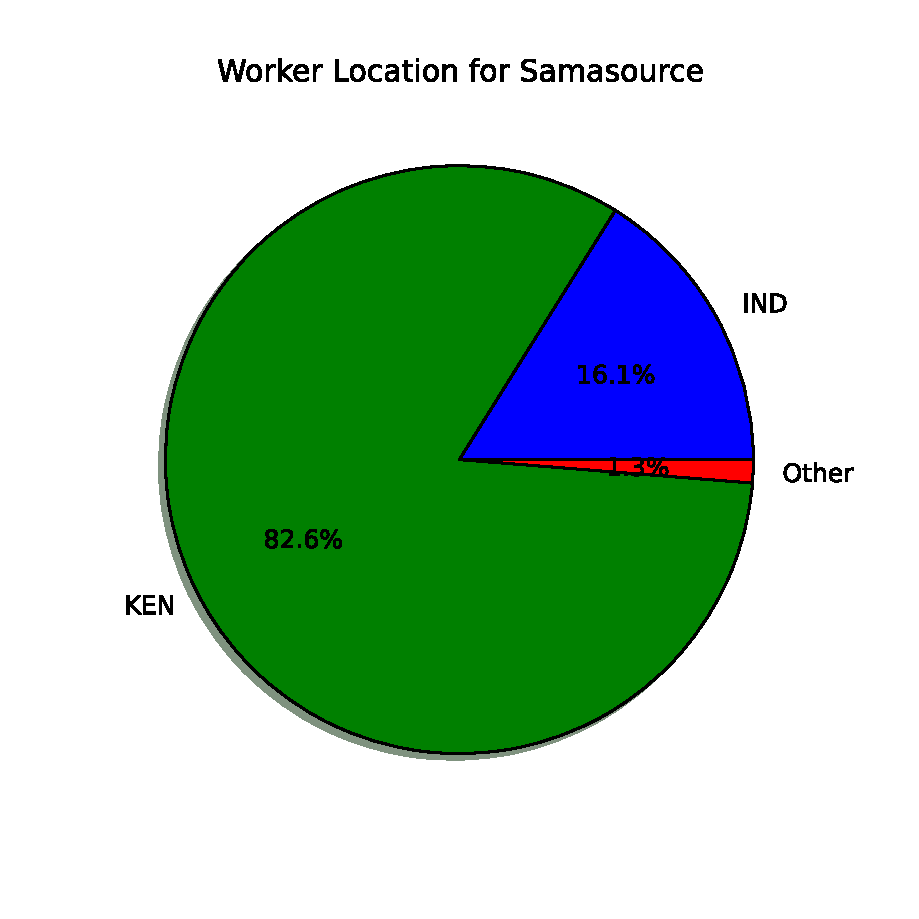
\includegraphics[width = 0.32 \columnwidth]{annotation/demog-sama.pdf}
\caption[Demographics of the worker pools.]{Demographics of the worker pools. AMT is Amazon Mechanical Turk. Each country has been abbreviated to its ISO 3166 code. GBR Great Britain, KEN Kenya, IND India, USA United States of America.}
\label{FigureCrowdDemographics}
\end{figure}

The annotation was performed by 711 participants who provided 79130 individual ratings. These were distributed across 527 video clips and 4 \ac{NVC} categories, with a total of 2108 questions. However, a significant proportion of the data was random, due to a significant proportion of uncooperative annotators. Three distinct worker pools were used. The internal worker pool is primarily the data previously collected and discussed in Section \ref{SectionAnalysisOfHumanAnnotation}, with the inclusion of further annotation by additional volunteers. In all, annotators from 33 countries participated in the annotation task. As can be seen in Figure \ref{FigureCrowdDemographics}, the demographics of each pool differ quite dramatically. Because the annotation data for a single annotator is usually sparse (meaning they are not required to complete every question in the survey), a significant amount of annotation is required for each culture before there is sufficient data to determine stable consensus vote ratings for every question. A considerable amount of annotation data was received from GBR (Great Britain), KEN (Kenya) and IND (India) and these cultures are used throughout the remainder of this thesis. The choice of these cultures is based on the need for distinct cultural groups of any origin, for which annotation data is available. The data from the USA was discarded, along with other cultures with a low level of participation, because the annotators of these cultures did not complete enough questions to form a complete set of results. With better targeting of annotation resources, it would be possible to greatly increase the number of distinct cultures.

The workers were divided into trusted and untrusted groups depending on their cooperation with the task. If the data is not filtered, the resultant labels are extremely noisy and are not appropriate for machine learning. The next section describes the filter method used to ensure the labels are of sufficient quality.

\subsection{Filtering Method}
\label{SectionAnnotationFilterMethod}

\begin{figure}
\centering
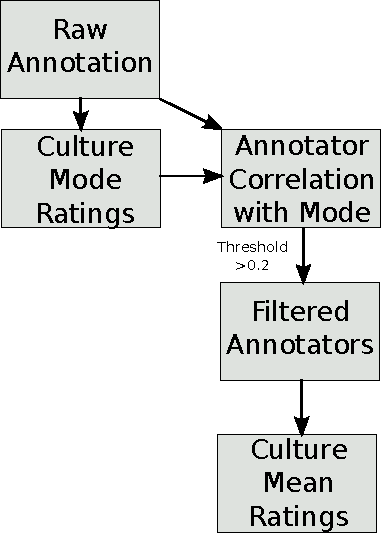
\includegraphics[width = 0.3 \columnwidth]{annotation/FlowAnnotationFiltering.pdf}
\caption[Flow chart of filtering method.]{Flow chart of filtering method. The statistical mode rating provides a robust standard by which annotators are assigned a trusted or untrusted score.}
\label{FigureFilterFlowChart}
\end{figure}

%There were three cultures for which a significant amount of data was collected: GBR, IND and KEN. 
Annotators were divided into two groups: trusted and untrusted. To achieve this, each worker's data $\singleAnnotatorRatings_{i, \nvcCategory} \in \mathbb{R}^{\numAnnotators \times 4}$ is compared to a robust rating standard $\robustAnnotation \in \mathbb{R}^{\numClips \times 4 \times 3}$. If a worker correlates with the robust standard to a sufficient degree, they are assigned to the trusted group and if not, the untrusted group (see Figure \ref{FigureFilterFlowChart}). The ratings for a single annotator $i \in \{0...\numAnnotators\}$ is found ($\clipId \in \{1...\numClips\}$):

\begin{gather}
\singleAnnotatorRatings_{i, \nvcCategory} = \{\ratingOfClip_j: (\ratingOfClip_j, \annotatorOfRating_j) \in \rawAnnotation_{\nvcCategory,\clipId}, \annotatorOfRating_j=i\} 
\end{gather}

Annotator $i$ is a member of culture $\textbf{c}_i \in \cultureList = \{GBR, KEN, IND\}$. In this chapter, the raw annotation data $\rawAnnotation$ refers to the cross cultural annotation data. The robust rating standard is based on the statistical mode $\modeFunc$ for clip $\clipId$ ratings, in \ac{NVC} category $\nvcCategory \in \setCategories$, $x \in \cultureList$:

\begin{gather}
\robustAnnotation_{\clipId,\nvcCategory,x} = \modeFunc(\{\ratingOfClip_i: (\ratingOfClip_i, \annotatorOfRating_i) \in \rawAnnotation_{\nvcCategory,\clipId}, \textbf{c}_i = x\})
\end{gather}

\begin{figure}
\centering
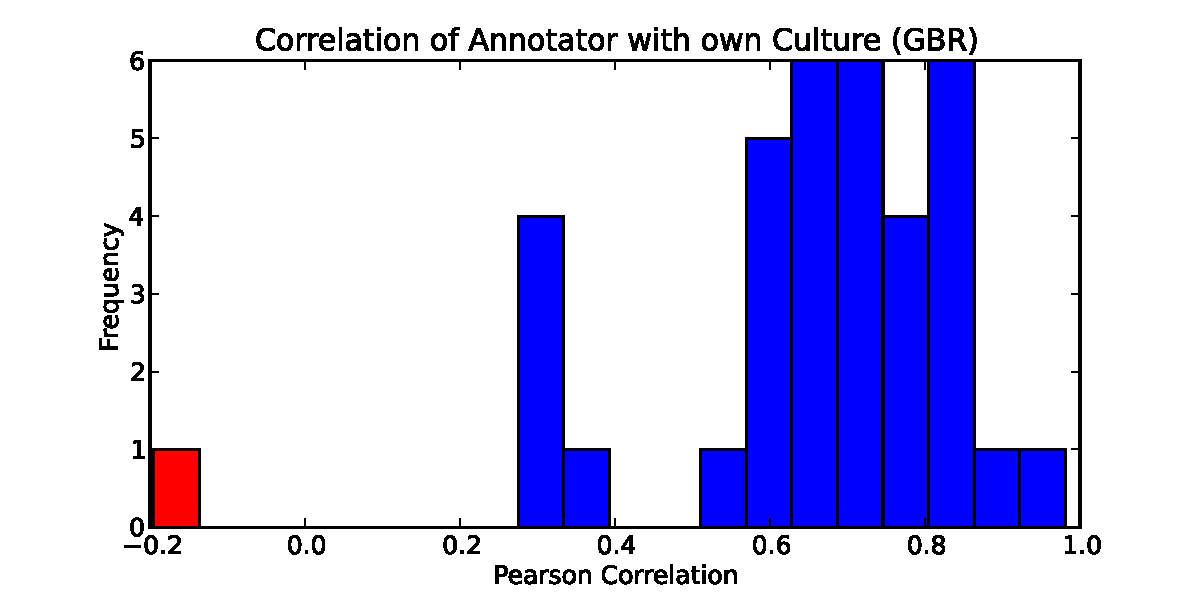
\includegraphics[width = 0.6 \columnwidth]{annotation/correlgbr.pdf}
\caption[Histogram of annotator correlation $\rho$ for GBR when compared to the robust ratings $\robustAnnotation$.]{Histogram of annotator correlation $\rho$ for GBR when compared to the robust ratings $\robustAnnotation$. Blue bars indicate annotators above the trusted threshold $\trustedThreshold$, and red bars indicate workers below. The majority of annotators in the GBR group have relatively good agreement with the robust rating.}
\label{FigureCorrelationHistOfGbr}
\end{figure}

\begin{figure}
\centering
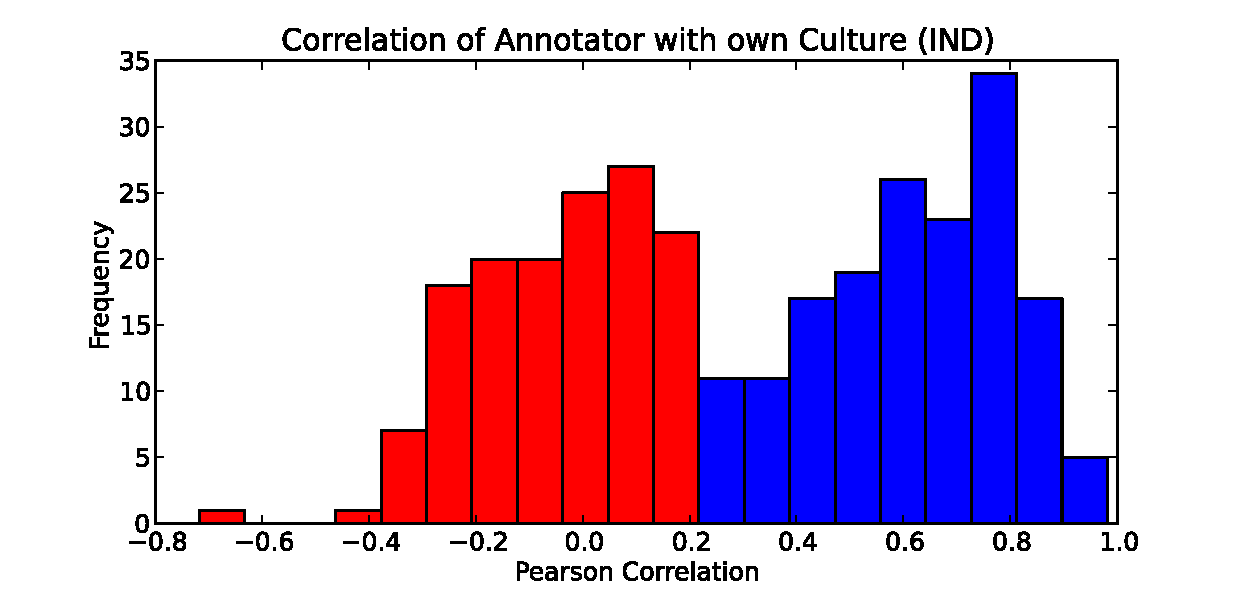
\includegraphics[width = 0.6 \columnwidth]{annotation/correlind.pdf}
\caption[Histogram of annotator correlation $\rho$ for IND when compared to the robust ratings $\robustAnnotation$.]{Histogram of annotator correlation $\rho$ for IND when compared to the robust ratings $\robustAnnotation$. Blue bars indicate annotators above the trusted threshold $\trustedThreshold$, and red bars indicate workers below. A significant number of workers in the IND group were assigned to the untrusted group.}
\label{FigureCorrelationHistOfInd}
\end{figure}

\begin{figure}
\centering
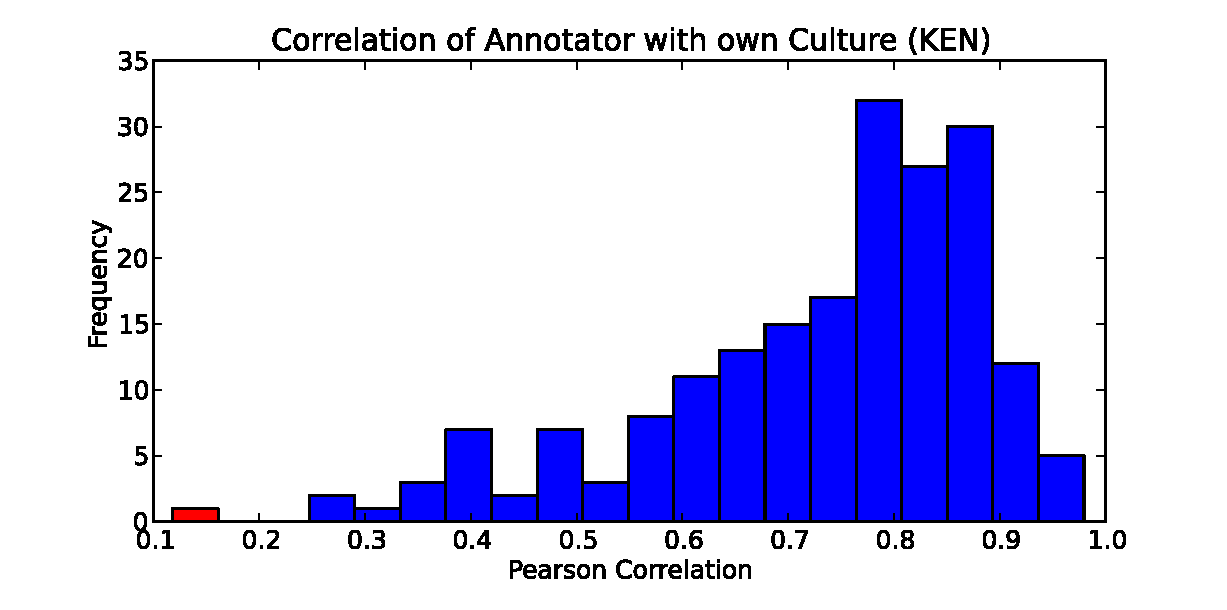
\includegraphics[width = 0.6 \columnwidth]{annotation/correlken.pdf}
\caption[Histogram of annotator correlation $\rho$ for KEN when compared to the robust ratings $\robustAnnotation$.]{Histogram of annotator correlation $\rho$ for KEN when compared to the robust ratings $\robustAnnotation$. Blue bars indicate annotators above the trusted threshold $\trustedThreshold$, and red bars indicate workers below. The majority of annotators in the KEN group have relatively good agreement with the robust rating.}
\label{FigureCorrelationHistOfKen}
\end{figure}

The statistical mode is used because it is relatively robust to uniformly distributed noise. Note that the raw annotation $\rawAnnotation$ is usually considered as a interval-scale, dimensional variable but here it is considered as a quantised variable. This is possible because the annotators' responses used a Likert scale with a finite number of options. Histograms of annotator correlation from the three cultures of interest are shown in Figures \ref{FigureCorrelationHistOfGbr}, \ref{FigureCorrelationHistOfInd} and \ref{FigureCorrelationHistOfKen}. As can be seen, there are cultural differences in the proportion of annotators assigned to the trusted and untrusted groups $\workerSet$. IND had a significant proportion of untrusted workers, while GBR and KEN were largely assigned to the trusted group. These perceptual cultural differences are probably more associated with the crowdsourcing worker pools. The vast majority of untrusted workers were in the Amazon Mechanical Turk pool, while annotators from the Samasource and Internal pools were largely trusted. A specific annotator $i$ provided ratings for a set of clips $\clipIndexAnnotated_i$. 
%The ratings $\rawAnnotation_{i}$ for each annotator $i$, having $\numRatingsForAnnotator_i$ across the 4 \ac{NVC} categories, are concatenated to form a combined ratings matrix $\crossCategoryRatings \in \mathbb{R}^{4 \numRatingsForAnnotator_i}$ ($\numRatingsForAnnotator \in \mathbb{N}^{\numAnnotators}$). The combined ratings are $\crossCategoryRatings$ compared to the robust standard $\robustAnnotation$ using Pearson correlation coefficient $\correlFunc$, $i \in \{0...\numAnnotators\}$:
Annotators only usually rate a subset of the corpus. The matrix of ratings by annotator $i$ is designated as $\widehat{\singleAnnotatorRatings}_{i,\nvcCategory} \in \mathbb{R}^{\clipIndexAnnotated_i \times 4}$, and the robust ratings that correspond with this clip subset is designated $\widehat{\robustAnnotation}_{i,\nvcCategory,x} \in \mathbb{R}^{\clipIndexAnnotated_i \times 4 \times 3}$:

\begin{gather}
\widehat{\robustAnnotation}_{i,\nvcCategory,x} = \{\robustAnnotation_{\clipId,\nvcCategory,x}: \clipId \in \clipIndexAnnotated_{i}\} \\
\widehat{\singleAnnotatorRatings}_{i,\nvcCategory} = \{ \singleAnnotatorRatings_{\clipId, \nvcCategory}: \clipId \in \clipIndexAnnotated_{i}\}
\end{gather}

The annotator ratings are then compared to the robust standard using Pearson correlation coefficient $\correlFunc$, $i \in \{0...\numAnnotators\}$. In this case, a 2{D} matrix, element wise Pearson correlation function $\correlFunc'$ to find correlation $\textbf{a}_i \in \mathbb{R}$ is used for convenience:

\begin{gather}
%\hat{\robustAnnotation_i} = {\robustAnnotation_{\nvcCategory,i}: \nvcCategory \in \setCategories}
\textbf{a}_{i} = \correlFunc'(\widehat{\singleAnnotatorRatings},\widehat{\robustAnnotation}_{\textbf{c}_i}) 
\end{gather}

Annotators that have a correlation above threshold $\trustedThreshold \in \mathbb{R}$ are assigned to the trusted set of workers:

\begin{gather}
%i \in \begin{cases}
%\workerSet_{trusted} : a_i \ge \trustedThreshold \\
%\workerSet_{untrusted} : a_i < \trustedThreshold
%\end{cases}
\workerSet_{trusted} = (\workerSet_{all,i} : \textbf{a}_{i} \ge \trustedThreshold) \\
\workerSet_{untrusted} = (\workerSet_{all,i} : \textbf{a}_{i} < \trustedThreshold)
\end{gather}

%If the correlation is above the trusted threshold $\trustedThreshold$, it is included in the set of trusted annotators $\workerSet_{trusted}$. 
A threshold value of $\trustedThreshold = 0.2$ was determined based on the minimum correlation of cooperative annotators from the GBR culture (Figure \ref{FigureCorrelationHistOfGbr}).
The final filtered annotation $\filteredAnnotation$ is computed by taking the statistical mean of trusted annotators. Trusted annotator ratings for a single question form a distribution. The mode only considers the peak of this distribution but disregards the other samples. However, using the mean is more sensitive to the overall views of the annotators. The mean is not a robust measure, which is why it is applied after the data is filtered:

\begin{gather}
\filteredAnnotation^{\clipId, \nvcCategory}_{\cultureSelect} = \overline{\{ \ratingOfClip_i : (\ratingOfClip_i, \annotatorOfRating_i) \in \rawAnnotation^{\clipId}_{\nvcCategory}, i \in \workerSet_{trusted} \}}
\end{gather}

%\begin{table}
%\centering
%\caption{Number of annotators and votes for cultures included in the unfiltered and filtered $\filteredAnnotation$ data set.}
%\begin{tabular}{ | c | c  c | c  c | }
%\hline
%Annotator & \multicolumn{2}{c|}{Num. Annotators} & \multicolumn{2}{c|}{Num. Ratings}  \\
%Country & Unfilter & Filter & Unfilter & Filter \\
%\hline
%\hline
%India & 304 & 167 & 37147 & 22754 \\
%Kenya & 196 & 195 & 15452 & 15420 \\
%GBR & 36 & 26 & 8211 & 8167 \\
%\hline
%\end{tabular}
%\label{NumFilteredWorkersTable}
%\end{table}

\begin{table}
\centering
\caption{Number of annotators and votes for cultures included in the unfiltered and filtered $\filteredAnnotation$ data set.}
\begin{tabular}{ | c || c | c  c || c | c  c | }
\hline
Annotator & \multicolumn{3}{c||}{Num. Annotators} & \multicolumn{3}{c|}{Num. Ratings}  \\
Country & Total & Trusted & Untrusted & Total & Trusted & Untrusted \\
\hline
\hline
India & 304 & 167 (55\%) & 137 & 37147 & 22754 & 14393\\
Kenya & 196 & 195 (99\%) & 1   & 15452 & 15420 & 32\\
GBR   & 36  & 26  (72\%) & 10  & 8211  & 8167  & 44\\
\hline
Total & 536 & 388 (72\%) & 358 (28\%) & 60810 & 46341 & 14469\\

\hline
\end{tabular}
\label{NumFilteredWorkersTable}
\end{table}

where $\cultureSelect \in \cultureList$. The quantity of annotations in the unfiltered $\rawAnnotation$ and filtered $\filteredAnnotation$ annotation sets are shown in Table \ref{NumFilteredWorkersTable}. The 28\% of users that were assigned to the untrusted group accounted for 23\% of the unfiltered data. This implies the trusted annotators answered a greater number of questions on average. After filtering, a significant amount of data remains available for use in training and evaluating machine learning techniques. Each annotator was assigned to a single culture by \ac{IP} address. This information allows a \culturallySpecific robust \ac{NVC} perception rating ($\robustAnnotation_{GBR}$,$\robustAnnotation_{IND}$,$\robustAnnotation_{KEN}$), which are used to filter annotators to form a final, culture specific, filtered annotation sets $\filteredAnnotation^{\clipId, \nvcCategory}_{GBR}$, $\filteredAnnotation^{\clipId, \nvcCategory}_{KEN}$ and $\filteredAnnotation^{\clipId, \nvcCategory}_{IND}$.

\thesiscomment{Is consensus just an artefact of filtering? Hair colour?}

%A method of finding a subset of trusted workers based on their mutual agreement has been described. 
Untrusted annotators were expected to provide uniformly random responses. Filtering the annotators to remove these responses was expected to result in a reduction in variance in the filtered data $\filteredAnnotation$ when compared to the unfiltered data $\rawAnnotation$. There is a possibility that a minority subset of self consistent annotators being selected and this would not represent an overall consensus. However, Table \ref{NumFilteredWorkersTable} shows that the majority of annotators are retained in the trusted set, which shows that this is not the case.

%Given the filtered data $\filteredAnnotation_{GBR}$, $\filteredAnnotation_{KEN}$ and $\filteredAnnotation_{IND}$, cultural differences between the annotators can be analysed. This analysis is performed in the following section.

\section{Analysis of Annotations}
\label{SectionAnalysisOfCultureAnnotation}

The previous section has described how the annotation data was collected from Internet workers and filtering was applied to obtain a high quality set of \ac{NVC} annotations. This annotation data describes the \ac{NVC} content for either \textit{agree}, \textit{thinking}, \textit{question} or \textit{understand} as observed from a particular culture (GBR, KEN or IND). However it is well known that \ac{NVC} perception is dependent on cultural rules and the specifics of cultural factors on \ac{NVC} perception is not well understood. This section provides a quantitative analysis as to the nature and extent of the cultural differences in the annotation data.

\thesisstatement{Annotation of NVC has a low inter-annotator agreement}

\thesisstatement{Different cultures have distinct patterns in their annotation results}

\begin{table}
\centering
\caption{Inter-culture correlation of filtered consensus data for different culture pairs. $\rho_{IND,KEN} = \correlFunc(\filteredAnnotation^{\clipId, \nvcCategory}_{IND},\filteredAnnotation^{\clipId, \nvcCategory}_{KEN})$. Individual annotators are not compared in this calculation but rather the overall cultural consensus.}
\begin{tabular}{ | c | c c c | }
\hline
 & India & Kenya & GBR \\
\hline
\hline
India & 1 & 0.56 & 0.55\\
Kenya &  & 1 & 0.64 \\
GBR    &  &  & 1 \\
\hline
\end{tabular}
\label{InterCultureCorrelationTable}
\end{table}

As can be seen in Table \ref{InterCultureCorrelationTable}, the correlation of pairs of cultures is at an intermediate level. A correlation value of less than one (corresponding to perfect correlation) was expected, because previous studies of emotion have observed cultural differences (see Section \ref{BackgroundCrossCulture}). A Pearson correlation above zero (corresponding to no correlation) implies \ac{NVC} perception in different cultures is not totally independent and a degree of commonality exists. This confirms our suspicion that \ac{NVC} perception is similar to emotion perception in that cultural differences exist, but there remains a significant commonality between cultures. Another point that is illustrated by Table \ref{InterCultureCorrelationTable} is that cultures have varying degrees of similarity to other cultures for perception of \ac{NVC}. The KEN-GBR correlation is higher than either IND-GBR or IND-KEN ($0.64$ vs. $0.56$ or $0.55$). This suggests that IND is the most distinctive in \ac{NVC} perception, and KEN-GBR are relatively similar. It might be expected that other cultures are much more or much less similar than the three cultures studied. This work was restricted to annotators with access to computer and Internet resources, but a broader examination of cultural differences would be interesting.

Pearson's correlation coefficient ignores scaling differences when comparing data. If cultures differed by only scaling differences, this would be ignored by the correlation measure. This is a desirable property, because scaling differences between cultures are relatively trivial to understand and model. However, less than perfect correlation scores indicate that annotation differences exist and they are not merely scaling differences.

\begin{figure}
\centering
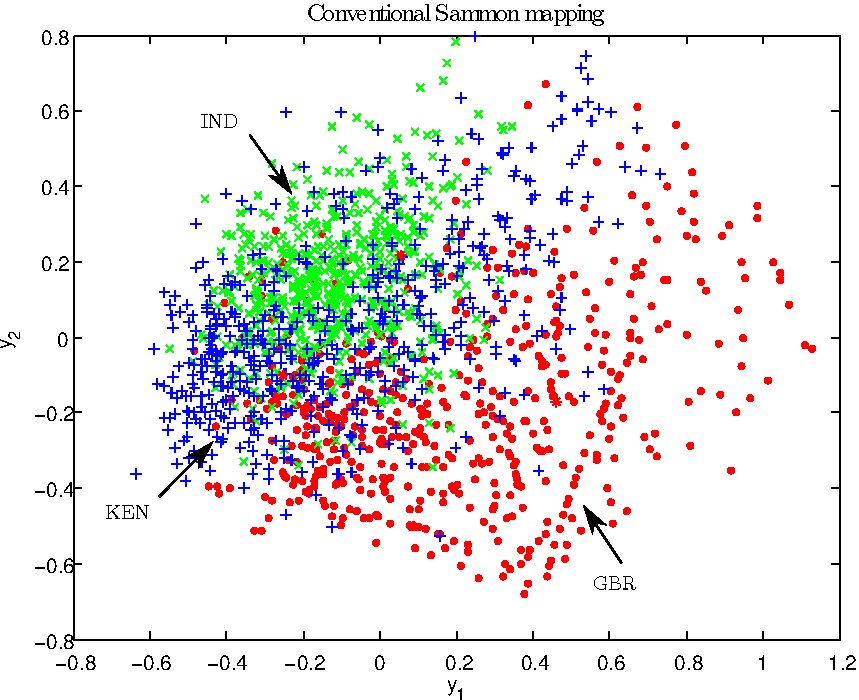
\includegraphics[width = 0.78 \columnwidth]{annotation/Sammon3Culture.pdf}
\caption[Sammon mapping of the filtered annotation responses.]{Sammon mapping of the filtered annotation responses. Each point represents the mean rating of a single clip within a single culture. The four \ac{NVC} categories are concatenated into a 4 component vector to enable distance pairs to be computed. GBR: red (.), IND: green (x), KEN: blue (+).}
\label{CultureSammonMapping}
\end{figure}

A way of visualising cultural differences in annotation of \ac{NVC} perception is the Sammon mapping \cite{Sammon1969}. This technique is a dimensionality reduction tool which maps high dimensional samples to a lower dimensional space while preserving inter-sample distances. For culture $\cultureSelect$, the filtered culture annotation $\filteredAnnotation^{\clipId, \nvcCategory}_{\cultureSelect}$ is a $527$ by $4$ matrix. The three filtered cultures  (GBR, IND, KEN) are combined into a $3 \times 527 = 1581$ by $4$ matrix. These points are transformed into a 2{D} space using Sammon mapping and plotted. This allows us to compare the distribution of annotation responses for different cultures. The result of this procedure is shown in Figure \ref{CultureSammonMapping}. This produces a complex distribution with some regions that are generally exclusive to a single culture, areas that are densely occupied by two overlapping cultures and one central zone where all cultures have a high density. The area of three culture overlap corresponds to annotation responses that appear in all cultures, the most common of which likely corresponds to ``no \ac{NVC} is being expressed''. Areas that are dominated by a single culture are interesting because they imply that for a subset of clips, a culture has provided a specific rating for the 4 \ac{NVC} categories that does not appear in the other cultures. This seems to be most apparent in the GBR annotations which has a significant proportion of points that are far from any other culture's points. This supports the idea that cultural differences in \ac{NVC} are not trivial to explain or model, and any mapping between \culturallySpecific annotation sets may be non-linear. 

\thesisstatement{People correlate better with their own culture consensus than with a global consensus}

\thesisstatement{Taking the global mean doesn't correspond to anything in real applications}

\begin{table}
\centering
\caption[Correlation of the mean annotator correlation within various cultures with their respective culture filtered annotation $\filteredAnnotation$ or the global Mean (taken as the combined India, Kenya and \ac{UK} ratings).]{Correlation of the mean annotator correlation within various cultures with their respective culture filtered annotation $\filteredAnnotation$ or the global Mean (taken as the combined India, Kenya and \ac{UK} ratings). Annotators correlate better on average with their own culture consensus than the global consensus $\globalAnnotation$.}
\begin{tabular}{ | c | c c c | }
\hline
 & India & Kenya & \ac{UK} \\
\hline
\hline
Own Culture Mean & 0.67 & 0.78 & 0.77 \\
Global Mean & 0.64 & 0.74 & 0.68 \\
\hline
\end{tabular}
\label{MeanAnnotatorCorrelationTable}
\end{table}

Because various filtering methods and mean ratings are used to arrive at the filtered annotations $\filteredAnnotation$, the extent the filtered annotations are representative of the individual annotator responses should be verified. Also, the validity of disregarding culture and the combining ratings to produce a global mean $\globalAnnotation$ can be considered.
%The filtered annotations is intended to represent the overall culture's \ac{NVC} perception and we should expect a annotator to be more similar to their respective culture, rather than a different culture. TESTS NOT DONE
These comparisons are shown in Table \ref{MeanAnnotatorCorrelationTable} and show an annotator's correlation to their own culture is relatively good. The lower correlation of IND may indicate a problem with data quality or perhaps there is greater perception individuality for this cultural group.
However, if cultural difference is ignored as in the case of global mean annotation $\globalAnnotation$, the individuals do not correlate as well as with their own culture consensus, in all three cases. Therefore, there is a divergence between individual annotators and the ratings that are intended to reflect them. Remember that taking a mean of a group of ratings is only valid if the annotators form a relatively self-consistent group. Therefore, ignoring culture produces a global annotation that has less validity. If global annotation data is used to train an automatic system, the labels that would be predicted would not necessarily correspond to any single annotator or any subset of annotators. This would not be compatible with the objective of producing an automatic system that would predict \ac{NVC} as a human would perceive \ac{NVC}.

\thesiscomment{DISCUSS differences exist other than culture and this is seen here, an area for further work}

\thesiscomment{DISCUSS When does the score converge? about 5 filtered votes?}

\thesiscomment{DISCUSS Any more ideas for analysis? Is there a way to map clusters from different cultures?}

%Conclusions are drawn in the next section, based on the experience of collecting data annotation and the results are analysed.

\subsection{Inter-annotator Agreement}
\label{SectionInterAnnotatorAgreement}

The annotation consensus score $\filteredAnnotation^{\clipId, \nvcCategory}_{\cultureSelect}$ is formed by taking the mean of trusted annotator ratings. This approach is only valid of sufficient annotators are in agreement with the label. Given that the annotator ratings are dimensional, the level of inter-annotator agreement can be determined by taking the standard deviation of ratings for each culture. A low standard deviation implies a high level of inter-annotator agreement. Figures \ref{FigureAgreementOfAnnotators1} and \ref{FigureAgreementOfAnnotators2} show the cumulative number of clips at various levels of agreement. As can be seen in these plots, some \ac{NVC} signals have a higher level of inter-annotator agreement (\textit{question}) and others have a lower level of agreement (such as \textit{thinking}). Different cultures are again seen to have an overall higher level of inter-annotator agreement (GBR) than others (IND). This may be caused by different levels of homogeneity in perception of \ac{NVC} for each culture.

A standard deviation of 0.289 corresponds to the level of agreement for random ratings (based on uniformly distributed ratings between 0 and 1). There are a significant number of \textit{thinking} \ac{NVC} examples that have a lower level of agreement than would be expected by change. This suggests that there may be more than one perception mode for \textit{thinking} \ac{NVC}, for at least some of the video clips in the corpus.

Section \ref{SectionRegressionHighAgreement} uses clips with a high level of inter-annotator agreement as the basis for regression. This addresses the issue that annotators sometimes do not agree enough to provide a meaningful label.

\begin{figure}
\centering
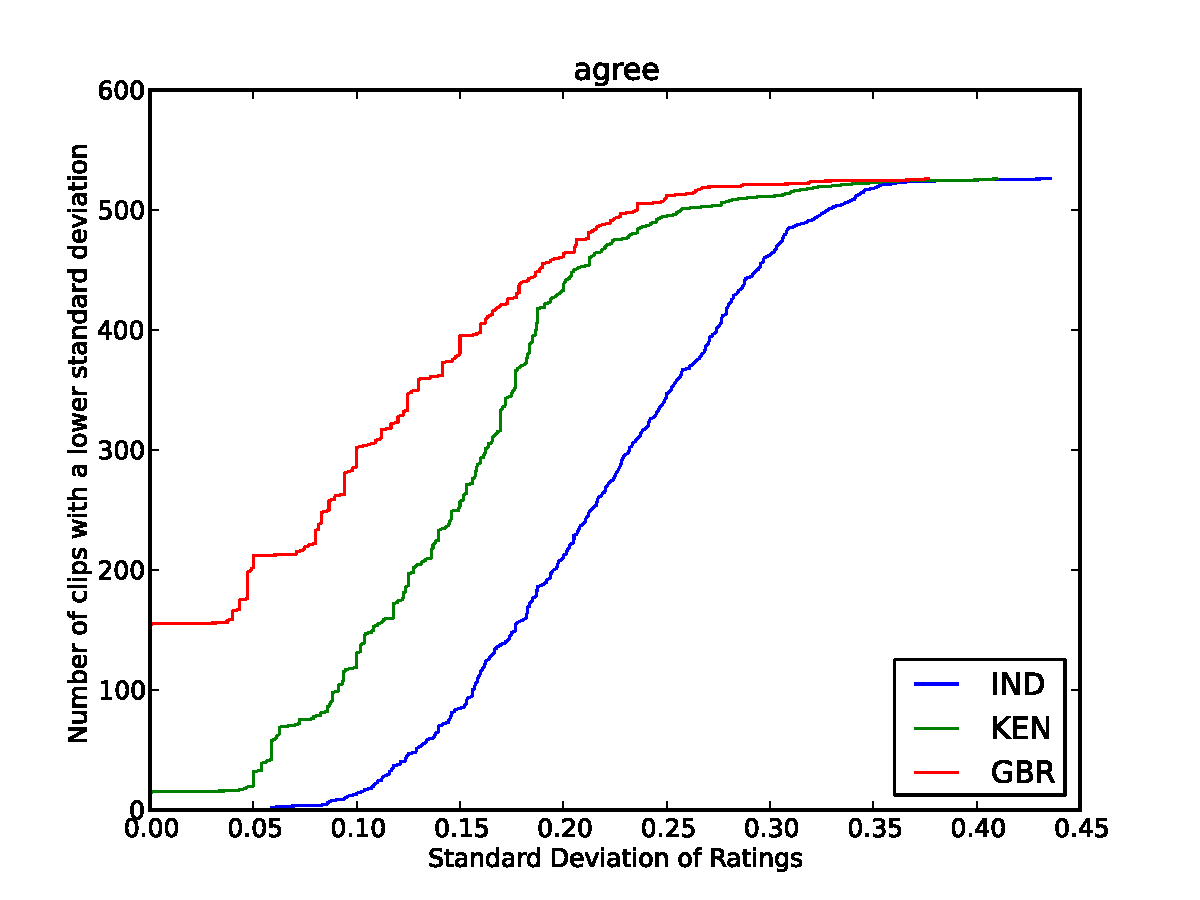
\includegraphics[width = 0.45 \columnwidth]{annotation/annotagree.pdf}
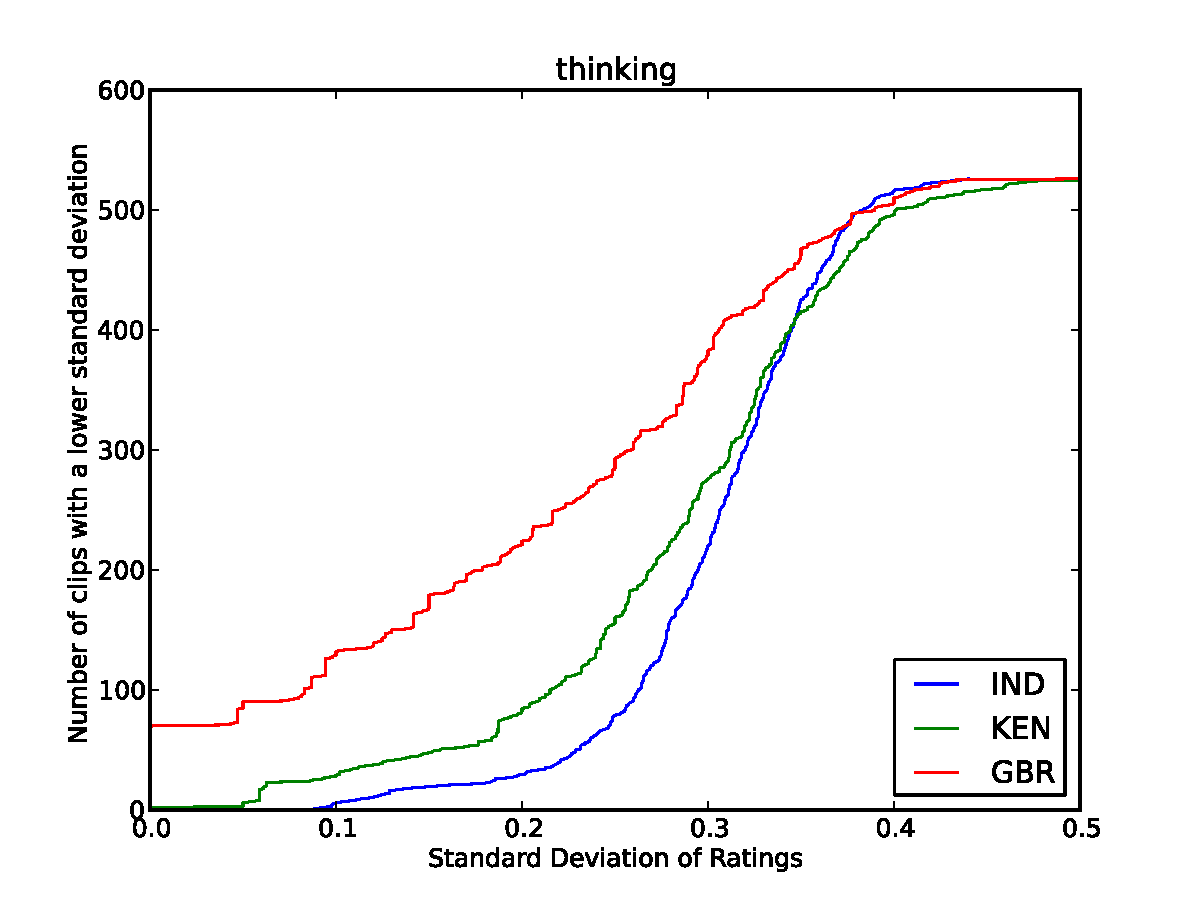
\includegraphics[width = 0.45 \columnwidth]{annotation/annotthinking.pdf}
\caption[Cumulative plot of the number of clips at various annotation standard deviations of annotator ratings.]{Cumulative plot of the number of clips at various annotation standard deviations of annotator ratings. Left plot shows \textit{agree} and the right plot shows \textit{thinking}.}
\label{FigureAgreementOfAnnotators1}
\end{figure}

\begin{figure}
\centering
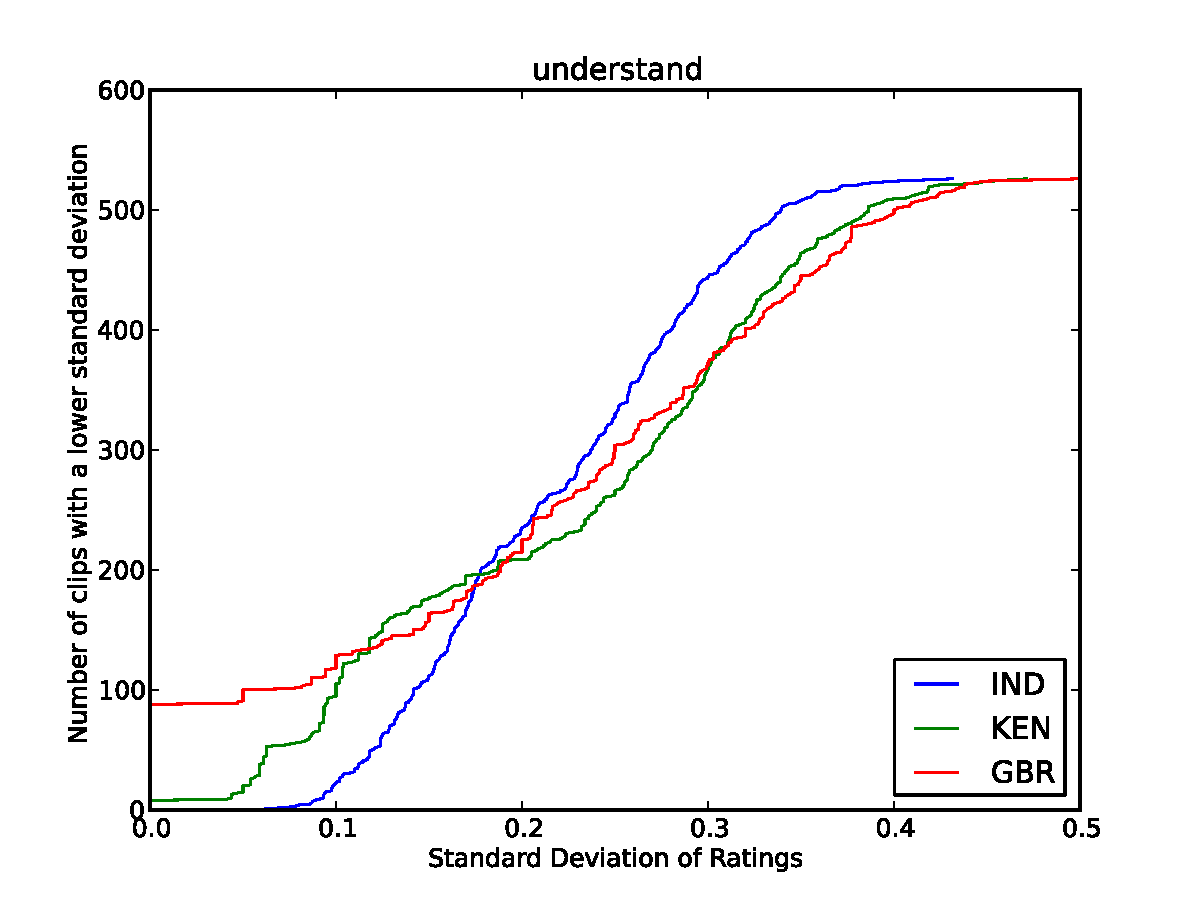
\includegraphics[width = 0.45 \columnwidth]{annotation/annotunderstand.pdf}
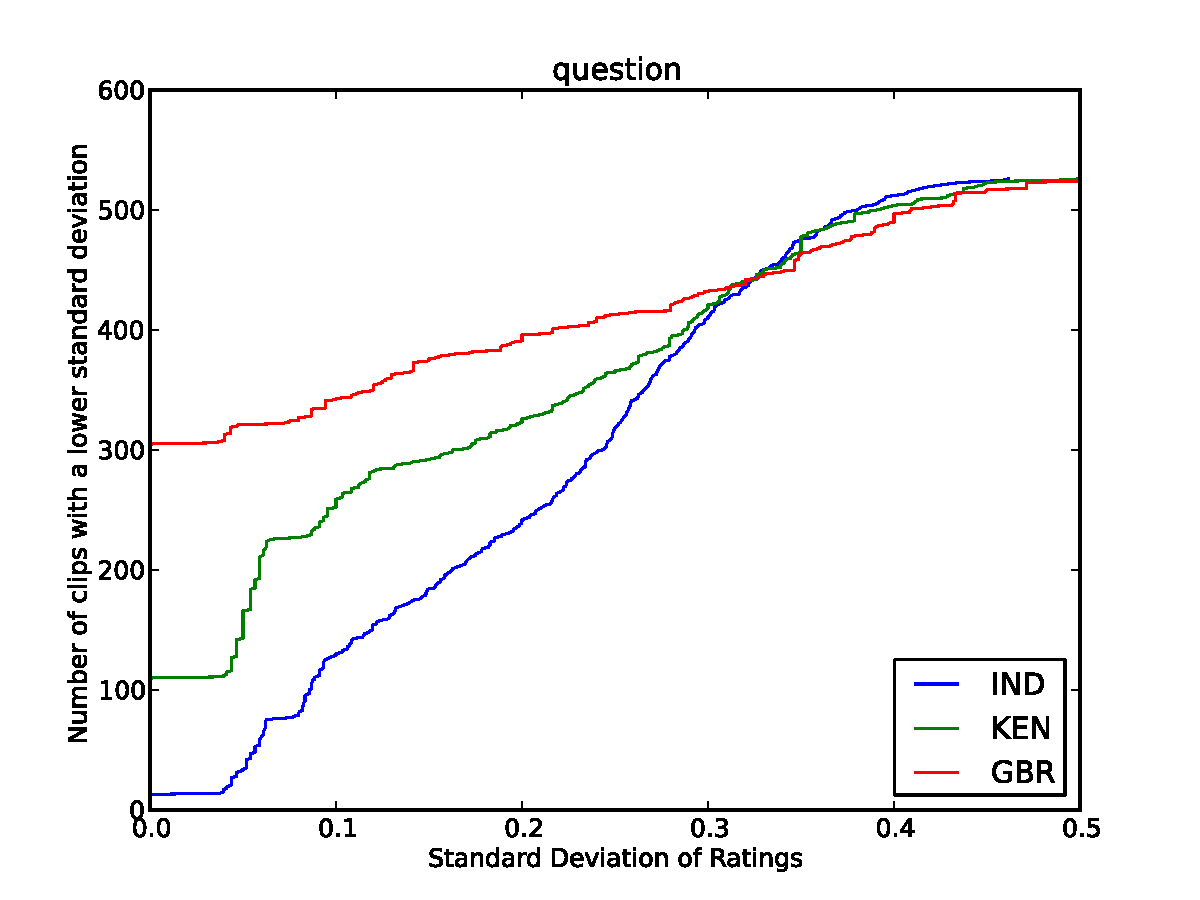
\includegraphics[width = 0.45 \columnwidth]{annotation/annotquestion.pdf}
\caption[Cumulative plot of the number of clips at various annotation standard deviations of annotator ratings.]{Cumulative plot of the number of clips at various annotation standard deviations of annotator ratings. Left plot shows \textit{understand} and the right plot shows \textit{question}.}
\label{FigureAgreementOfAnnotators2}
\end{figure}

\section{Conclusion}

\thesiscomment{DISCUSS If we have much more data, we could use unsupervised clustering without needing demographics. Or demographics can assist in semi-supervised clustering.}

This chapter has described the collection of cross cultural \ac{NVC} perception data. The data was collected based on paid Internet workers from multiple cultures. Because some workers did not cooperate with the task, the data was filtered to isolate the valid annotation data. The annotations were analysed and found to contain differences that were not merely linear scaling effects. This video annotation resulted in a new, cross cultural annotation of \ac{NVC} on natural informal conversations. The annotation data has been publicly released for further use. This helps to address the lack of publicly available \ac{NVC} annotation data. 

Crowdsourcing annotation data may prove to be a significant resource in human behaviour understanding if the quality issues can be addressed. The quality assurance tools that are currently available focus on annotation of discrete, objective labels. These objective labels are appropriate for computer vision tasks such as object recognition where the concepts are well defined. 
%An example question for object recognition can be as simple as a binary choice, e.g. ``Is there are car in this photograph?''. 
%Any disagreement in annotators usually indicates that the minority view is incorrect, based on the assumption that untrusted workers provide random responses rather than trying to sabotage the annotation exercise. 
However, discrete label filtering method is not useful in subjective tasks, such as \ac{NVC} annotation. In this case, inter-annotator disagreements do not necessarily imply that some of the annotators are wrong. Quality is still a significant concern and the filtering method proposed in this chapter is a step towards addressing this. The filtering method does rely on using the annotation mode, which depends on sufficient annotator participation to form a stable result. Also, the annotators are hard assigned to trusted and untrusted groups. It may be more efficient to use soft assignments for annotator trust.

The presence of cultural perception differences is not particularly surprising given a similar effect is often observed in emotion. The significance of the findings in this chapter is the confirmation of \ac{NVC} annotation differences and a quantitative analysis of the differences. The results suggest that different cultures have varying degrees of similarity. These perceptual cultural similarities might be exploited to reduce the number of \culturallySpecific perception models needed for \ac{NVC} recognition, possibly by treating actual annotator group perceptions as a mixture of two or more exemplar perception models.

There are significant shortcomings of Internet crowdsourcing for studying perception. The annotators are not screened and the environment in which the annotation is performed is not controlled. Each culture has a different availability of computer resources, different levels of computer literacy, different demographics that will undertake the task and the annotation is performed in different settings. These differences are known to be a factor in emotion perception and are likely to play a role in \ac{NVC} perception. The use of demographic questions may allow some of these variables to be controlled. This chapter has used English language questionnaires, but there can be cultural differences in the understanding of language. Given that perception differences in this chapter may be caused by either language perception differences or \ac{NVC} perception differences, it is hard to distinguish these effects. One possible method to check and possibly quantify language differences in crowdsource annotation is to conduct cross cultural annotation of data that has objective labels, using a single language questionnaire. If the annotators were consistent across cultures, this result would validate the approach of using a single language. Translation of \ac{NVC} survey instruments replaces the uncertainty of language perception with uncertainty over the validity of the translation of \ac{NVC} concepts, which by definition do not directly correspond to word based concepts.

%Emotion is studied by examining the response to an emotionally inducing stimuli. However, \ac{NVC} focuses on conscious action, rather than automatic reaction. It is possible that culturally equivalent stimuli do not exist for \ac{NVC}.

The next chapter uses this \continuous annotation data to approach the \ac{NVC} recognition problem by cross cultural regression.
